\selectlanguage{italian}%

\section{Simulazione}

\begin{figure}[H]
	\centering
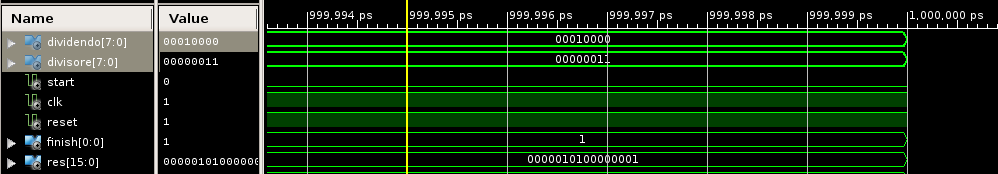
\includegraphics[scale=0.5]{esercizio14/images/div_restoring_tesbench.png}
	\caption{Esempio divisione}
\end{figure}

Il quoziente ed il resto vengono espresse in un unica stringa da 16
bit dove la met� superiore della stringa � il quoziente la met� inferiore
il resto, questo per facilitare successivamente la scrittura sul display.\selectlanguage{italian}%

